\documentclass{article}
\usepackage{graphicx}
\usepackage{amsmath}
\usepackage{float}
\usepackage[margin=1in]{geometry}

\DeclareMathOperator{\length}{length}

\begin{document}
\title{Single Source Shortest Path on 2D-Grid with Breath First Search in Python 3}
\author{Brandon Tang}
\maketitle

\begin{abstract}
    Given a fixed 2D maze of empty and walled cells, we demonstrate the usage of breadth first search to determine the shortest path between a fixed starting cell and a variable target cell.
\end{abstract}

\section{Introduction}

    \subsection{Problem Statement}
    The problem of finding the shortest path on a 2D grid is very fundamental problem in graph theory. In this project, we are given a set maze in the form of a text file of boolean values. A value of \texttt{True} represents that a cell that is a wall while a value of \texttt{False} represents an empty cell. The boolean values are ordered to produce a maze when interpreted correctly.

    We are also given a fixed starting and ending cell, the coordinates of which we are to interpret ourselves from the given image of the maze in the figure \ref{fig:problem_maze}. The destination cell is a variable that our program should be able to construct a path to. Adjacent cells along this path must always be empty and either to the left, right, top or bottom of another cell.

    The eventual output should be a 2D colour map outlining the shortest path from the starting to the destination cells. This is expected to be produced using the library \texttt{matplotlib.pyplot}.

    \begin{figure}[H]
        \centering
        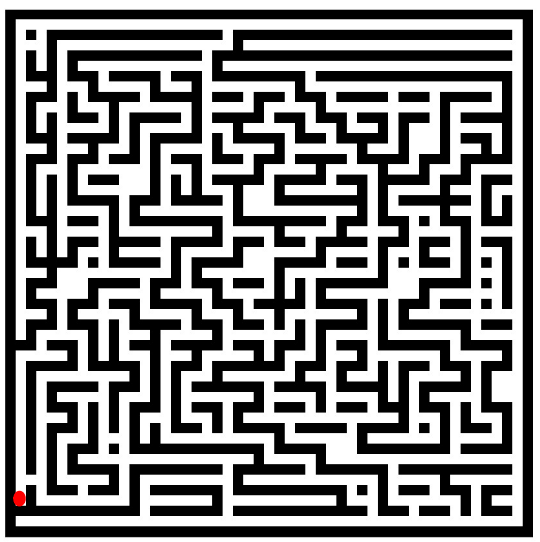
\includegraphics[width=0.5\textwidth]{img/problem_statement_maze.png}
        \caption{Maze image in problem statement with red dot as starting cell}
        \label{fig:problem_maze}
    \end{figure}

\section{Methodology}
    \subsection{Parsing the Maze}
    Without any knowledge of how the boolean values are ordered, we assumed a standard row-major representation of the maze file.

    This is parsed into a 2D python list in 3 steps.

    Firstly, we simply read the file line by line to form a 1D list ($l_1$). Each element is a boolean value attained by using the \texttt{eval()} function on their equivalent string versions. Secondly, we determine the length of each size of the maze. From the image, we hypothesize that the maze is square in shape. Thus, we determine the maze length $maze_l = \sqrt{\length({l_1})}$. Thirdly, we set the value of the cell at $(r, c)$ to be equal to the element in position $r \times maze_l + c$ in $l_1$.

    After this effort, we visualised this maze but realised that our version of the maze was a tranpose of the one in the problem statement, indicating that the maze was actually in column-major representation instead, thus we did a simple tranpose to correct the orientation as seen in Figure \ref{fig:parsed_maze}.

    \begin{figure}[H]
        \centering
        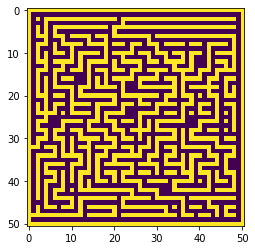
\includegraphics[width=0.5\textwidth]{img/parsed_maze.png}
        \caption{Parsed Maze}
        \label{fig:parsed_maze}
    \end{figure}


    \subsection{Single Source Shortest Path Algorithm}
    There exist several different (efficient approaches to solve the single source shortest path (SSSP) problem.

    \begin{itemize}
        \item Breadth First Search (BFS)
        \item Dijkstra
        \item A*
    \end{itemize}

    What affected our selection of the algorithm was the fact that the grid represented an \textbf{unweighted} graph. This means that BFS provides a valid solution since the distance of a path is always equal to the number of nodes along the path, indicating that it is not possible for any relaxation operations\footnote{A relaxation operation from nodes u to v through k refers to checking if the distance from u to v is reduced if we go to from u to k and then to v.}.

    When applied on an unweighted graph, Dijkstra visits the nodes in the same order as BFS. However, due to the use of a binary heap or binary search tree (BST) instead of a queue, there is an extra logarithmic factor in its time complexity. This results in a slower O($V \log V$) complexity\footnote{Dijkstra has a time complexity of O($E \log V$) when applied with a binary heap or BST, however, since the degree of each vertex in a grid is always 4, $E \propto V$ thus O($E \log V$) = O($V \log V$)} compared to the O($V$) complexity of BFS.

    It is possible that A* could have faster run time over BFS due to the reduced number of states visited. However, given the large number of long contiguous walls, A* will likely still have to check a large number of cells. This is assuming that we use the Euclidean distance between each cell and the target cell as the heuristic.

    As such, we opt to use the simpler and yet optimal BFS algorithm. This algorithm determines the distance from the source cell to all cells and records it a 2D \texttt{numpy} array. This can be visualised in Figure \ref{fig:dist_array}.

    \begin{figure}[H]
        \centering
        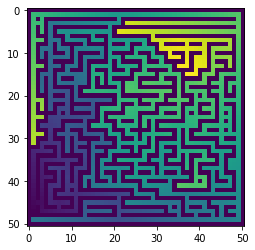
\includegraphics[width=0.5\textwidth]{img/dist_array.png}
        \caption{Maze with cells coloured by distance from source}
        \label{fig:dist_array}
    \end{figure}

    \subsection{Backtracking to Determine Optimal Path}
    Having found the minimum distance to each cell, we now need to determine the path and plot it. Here, we opt to do so with a backtracking algorithm. Starting with \texttt{(r,c)} being the target cell, we recusively use the following relation.

    \begin{verbatim}
        (r, c) = (nr, nc) such that
        dist[nr][nc] = min(dist[x][y]) for all adjacent (x,y) to (r,c)\end{verbatim}

    As we backtrack, we store \texttt{(r,c)} is a list. This stops when \texttt{(r,c)} reaches the source cell. Then, we reverse the list and plot the path on a new array.

    For better visualisation, we also plot the walls of the maze onto this new array, but with a lower brightness value.

    \begin{figure}[H]
        \centering
        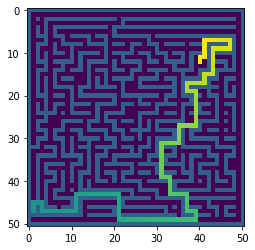
\includegraphics[width=0.5\textwidth]{img/solved_maze.png}
        \caption{Maze with path to destination (12, 40)}
        \label{fig:solved_maze}
    \end{figure}

    \section{Alternative Ideas}
    \subsection{Parent Array}
    Instead of backtracking, we could have stored the parent\footnote{the parent of cell \texttt{(nr, nc)} is the last cell along the path to \texttt{(nr, nc)}.} to each cell in another 2D array and updated it everytime we pushed the new cell into the queue during the BFS. This would allow for much faster backtracking if the nodes had a larger degree since it would allow for O($V$) rather than O($E$) backtracking.
    
\end{document}